\begin{table}[htbp]
\caption{Finite-sample experiment: 200 replications per cell. FWER is the frequency of any false strict order. Hub columns report certification of vertex zero as uniquely first; null cells have no unique population hub.}\label{tab:exact}
\centering\small
\begin{tabular}{rlrrrr}
\toprule
$p$ & Model & $n$ & Order FWER & Hub: order & Hub: box \\
\midrule
12 & Discrete null & 252 & 0.025 & --- & --- \\
12 & Discrete null & 1008 & 0.030 & --- & --- \\
12 & Gaussian star & 252 & 0.020 & 0.000 & 0.000 \\
12 & Gaussian star & 1008 & 0.010 & 0.000 & 0.000 \\
12 & Gaussian star & 4096 & 0.000 & 1.000 & 0.000 \\
12 & Independence & 252 & 0.000 & --- & --- \\
12 & Independence & 1008 & 0.030 & --- & --- \\
12 & Independence & 4096 & 0.070 & --- & --- \\
12 & Near tie & 252 & 0.005 & 0.000 & 0.000 \\
12 & Near tie & 1008 & 0.000 & 0.000 & 0.000 \\
12 & Near tie & 4096 & 0.000 & 0.000 & 0.000 \\
12 & $t_5$ star & 252 & 0.000 & 0.000 & 0.000 \\
12 & $t_5$ star & 1008 & 0.010 & 0.000 & 0.000 \\
12 & $t_5$ star & 4096 & 0.000 & 1.000 & 0.000 \\
52 & Gaussian star & 252 & 0.000 & 0.000 & 0.000 \\
52 & Gaussian star & 4096 & 0.000 & 0.790 & 0.000 \\
52 & Independence & 252 & 0.035 & --- & --- \\
52 & Independence & 4096 & 0.035 & --- & --- \\
52 & Near tie & 252 & 0.000 & 0.000 & 0.000 \\
52 & Near tie & 4096 & 0.005 & 0.000 & 0.000 \\
52 & $t_5$ star & 252 & 0.015 & 0.000 & 0.000 \\
52 & $t_5$ star & 4096 & 0.010 & 0.780 & 0.000 \\
\bottomrule
\end{tabular}
\end{table}
Across the finite-sample cells, the smallest observed simultaneous degree coverage was 0.995, and the smallest rank coverage was 1.000. The largest observed false-order frequency was 0.070 (14/200), in the $p=12$, $n=4096$ Independence cell; its Wilson 95\% interval is [0.042, 0.114]. A Monte Carlo proportion above 0.05 is not itself a contradiction of the finite-sample theorem. We report it rather than truncating observed errors at the nominal level.

Figure~\ref{fig:power} distinguishes hub certification from complete-tree recovery in the separated models. The full-sample rectangular baseline certified no hub at the displayed sample size. Successful hub inference need not imply that every edge is forced. Conversely, the short-sample and near-tie cells largely remain unresolved. A condition based on four uniform-band half-widths exceeding a tree separation margin is a sufficient recovery condition; failure of that condition is not an impossibility result for all Kendall methods.
\begin{figure}[htbp]\centering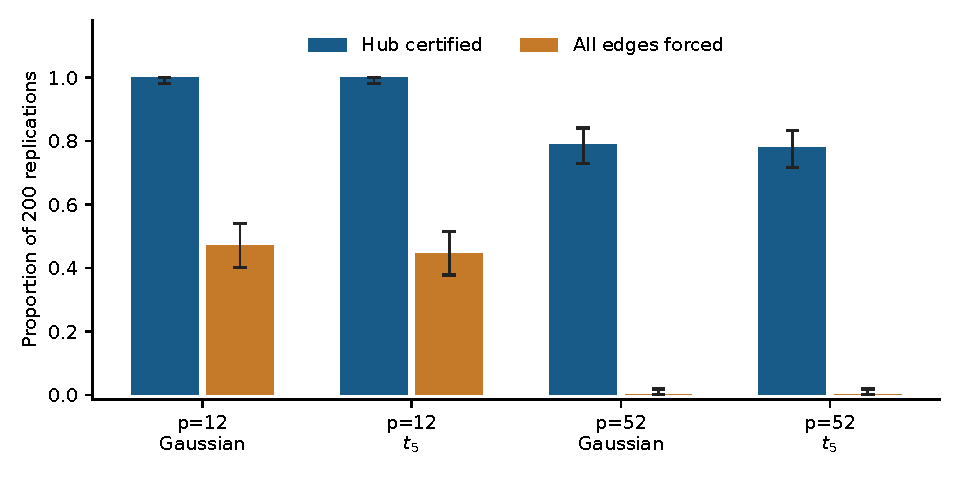
\includegraphics[width=\textwidth]{Fig_power.pdf}\caption{Certification at $n=4096$, from 200 replications per cell. Hub certification uses the upper rank endpoint; full recovery requires all $p-1$ edges to be forced by screening. Whiskers are Wilson 95\% Monte Carlo intervals. The Hoeffding-box hub rate is zero in all four cells.}\label{fig:power}\end{figure}
